
\documentclass[12pt,epsfig,color,russian]{article}
\usepackage[russian]{babel}
\usepackage{epsfig}
\usepackage{color}

\topmargin=0cm
\hoffset -30mm
\voffset -12mm
\setlength{\unitlength}{1mm}
\parindent=10mm
\textheight=250mm
\textwidth=185mm
\pagestyle{empty}

\begin{document}
\sf\Large


\centerline{\underline{\Huge\bf ДВИЖЕНИЕ ТВЕРДОГО ТЕЛА}}

Как уже говорилось, любое движение = поступательное + вращение.\\
\underline{\bf Поступательное}: все точки тела имеют равные $\vec{v}$ и равные $\vec{a}$. Если мысленно разбить тело на кусочки, то $\forall \Delta m_i$ по 2зН: $\Delta m_i\cdot\vec{a}=\vec{f_i}+\vec{F_i}$, где $\vec{f_i}$ -- внутренние силы от других элементов тела, а $\vec{F_i}$ -- силы внешние. По 3зН: $\sum \vec{f_i}=0$, поэтому
\begin{displaymath}
\sum_i\Delta m_i\cdot\vec{a}=\sum_i\vec{F_i}\hspace{10mm}\Rightarrow\hspace{10mm}
\vec{a}\cdot\sum_i\Delta m_i=\sum_i\vec{F_i}\hspace{10mm}\Rightarrow\hspace{10mm}
M\cdot\vec{a}=\vec{F}
\end{displaymath}
$\vec{F}=\sum\vec{F_i}$ -- {\bf главный вектор внешних сил}.\\[2mm]
\fbox{\parbox{190mm}{\begin{center}\color{blue}
Рассмотрение поступательного движения твердого тела можно заменить рассмотрением движения одной материальной точки с массой тела, находящейся под действием главного вектора внешних сил.
\end{center}
}}\\

При более сложном (непоступательном) движении: {\bf разные} точки тела имеют {\bf разные} скорости $\vec{v_i}$ и {\bf разные} ускорения $\vec{a_i}$.\\
  \begin{picture}(190,45)(0,0)
   %\put(0,0){\framebox(190,40)[b]{}}
   \put(85,0){\includegraphics{GP005F01.eps}}
   \put(0,0){\makebox(0,0)[bl]{\parbox{80mm}{Пример: на этом повороте левые колеса проезжают больший путь, чем правые $\Rightarrow$ водитель движется с большей скоростью, чем пассажир!
   }}}
  \end{picture}\\[10mm]
Разбив (мысленно) тело на малые кусочки, для каждого кусочка получим:
\begin{displaymath}
 \Delta m_i\cdot\vec{a_i}=\vec{f_i}+\vec{F_i}
\end{displaymath}
Если просуммировать и учесть, что $\sum \vec{f_i}=0$, а $\sum\vec{F_i}=\vec{F}$, то
\begin{equation}
\sum_i\Delta m_i\cdot\vec{a_i}=\sum_i\vec{F_i}=\vec{F}
\end{equation}
но тут уже все $\vec{a_i}$ -- разные, и их из-под знака $\sum$ не вынести... Что делать?
\fbox{\parbox{190mm}{\begin{center}\color{blue}
{\bf Центр масс $\equiv$ центр инерции $\equiv$ центр тяжести}: ($\cdot$)C
\begin{displaymath}
x(C)=\frac{\sum x_i\cdot\Delta m_i}M\hspace{10mm}
y(C)=\frac{\sum y_i\cdot\Delta m_i}M\hspace{10mm}
z(C)=\frac{\sum z_i\cdot\Delta m_i}M
\end{displaymath}
\begin{displaymath}
x(C)=\int x\,\rho\,dV/M \hspace{10mm}
y(C)=\int y\,\rho\,dV/M\hspace{10mm}
z(C)=\int z\,\rho\,dV/M
\end{displaymath}
\end{center}
}}\\[2mm]
Если тело C состоит из частей A+B, то его центр масс совпадает со средне-взвешенным от центров масс отдельных частей:
\begin{displaymath}
\vec{r}(C) =\frac{m_A\cdot\vec{r}(A)+m_B\cdot\vec{r}(B)}{m_A+m_B}
\end{displaymath}


Ускорение центра масс $\vec{a}(C)$ по составляющим:
\begin{displaymath}
a_x(C) \equiv \frac{d^2x(C)}{dt^2}
=\frac{d^2}{dt^2}\left(\frac{\sum x_i\cdot\Delta m_i}M\right)
=\frac{\sum \Delta m_i\cdot\frac{d^2x_i}{dt^2}}M
=\frac{\sum \Delta m_i\cdot a_{ix}}M
\end{displaymath}
\begin{displaymath}
a_y(C) \equiv \frac{d^2y(C)}{dt^2}
=\frac{d^2}{dt^2}\left(\frac{\sum y_i\cdot\Delta m_i}M\right)
=\frac{\sum \Delta m_i\cdot\frac{d^2y_i}{dt^2}}M
=\frac{\sum \Delta m_i\cdot a_{iy}}M
\end{displaymath}
\begin{displaymath}
a_z(C) \equiv \frac{d^2z(C)}{dt^2}
=\frac{d^2}{dt^2}\left(\frac{\sum z_i\cdot\Delta m_i}M\right)
=\frac{\sum \Delta m_i\cdot\frac{d^2z_i}{dt^2}}M
=\frac{\sum \Delta m_i\cdot a_{iz}}M
\end{displaymath}\\
или сразу в векторном виде:
\begin{displaymath}
\vec{a}(C) \equiv \frac{d^2\vec{r}(C)}{dt^2}
=\frac{\sum \Delta m_i\cdot \vec{a}_{i}}M
\end{displaymath}

Сравнивая с (1), получаем: \hspace{10mm}$M\vec{a}(C) =\vec{F}$
\\[3mm]
\fbox{\parbox{190mm}{\begin{center}\color{blue}
Центр масс (ц.м.) тела движется так, как движется материальная точка с массой, равной массе тела, под действием силы, равной главному вектору внешних сил.
\end{center}
}}\\[1mm]

Если $\vec{F}$=0, то ц.м. покоится (или движется прямолинейно и равномерно).

Внутренние силы не могут изменить движение ц.м.
\newpage
\noindent
\begin{tabular}{|cc||cc|} \hline
\multicolumn{2}{|c||}{\rule[-5mm]{0mm}{13mm}\bf Поступательное движение} &
\multicolumn{2}{c|}{\bf Вращательное движение}\\ \hline\hline
\multicolumn{4}{|c|}{\color{blue}\bf Физические величины и понятия:\rule[-5mm]{0mm}{15mm}}\\ \hline
расстояние \rule[-5mm]{0mm}{13mm}& $s$ & угол & $\varphi$\\ \hline
координата \rule[-5mm]{0mm}{13mm}& $\vec{s}$ & угол & $\vec{\varphi}$\\ \hline
скорость \rule[-5mm]{0mm}{13mm}& $\vec{v}=\dot{\vec{s}}$ & угловая скорость & $\vec{\omega}=\dot{\vec{\varphi}}$\\ \hline
ускорение \rule[-5mm]{0mm}{13mm}& $\vec{a}=\ddot{\vec{s}}$ & угловое ускорение & $\vec{\beta}=\ddot{\vec{\varphi}}$\\ \hline
масса \rule[-5mm]{0mm}{13mm}& $m$ & момент инерции & $\mathcal{I}=mr^2$\\ \hline
кол.дв. (импульс)\rule[-5mm]{0mm}{13mm}&$\vec{p}=m\vec{v}$ & момент импульса & $\vec{\mathcal{L}}=\left[\vec{r}\times\vec{p}\right]=\mathcal{I}\vec{\omega}$ \\ \hline
сила \rule[-5mm]{0mm}{13mm}&$\vec{f}$ & момент силы & $\vec{\mathcal{M}}=\left[\vec{r}\times\vec{f}\right]$ \\ \hline
импульс силы \rule[-5mm]{0mm}{13mm}&$\vec{f}\Delta t$ & импульс момента силы & $\vec{\mathcal{M}}\Delta t$ \\ \hline
кин.энергия \rule[-5mm]{0mm}{13mm}&$E_k=\frac{mv^2}2$ & энергия вращения &
$\mathcal{E}_{\mathrm{rot}}=\frac{\mathcal{I}\omega^2}2$ \\ \hline\hline
\multicolumn{4}{|c|}{\color{blue}\bf Законы сохранения для изолированной системы:\rule[-5mm]{0mm}{15mm}}\\ \hline
импульса\rule[-5mm]{0mm}{13mm}&$\vec{p}=$const&
момента импульса&$\vec{\mathcal{L}}=$const\\ \hline\hline
\multicolumn{4}{|c|}{\color{blue}\bf Второй закон Ньютона:\rule[-5mm]{0mm}{15mm}}\\ \hline
\multicolumn{2}{|c||}{\rule[-5mm]{0mm}{13mm}$\vec{f}\Delta t = \Delta(\vec{p})$}&
\multicolumn{2}{c|}{$\vec{\mathcal{M}}\Delta t = \Delta(\vec{\mathcal{L}})$}\\ \hline
\multicolumn{2}{|c||}{\rule[-5mm]{0mm}{13mm}$\vec{f} = m\vec{a}$}&
\multicolumn{2}{c|}{$\vec{\mathcal{M}} = \mathcal{I}\vec{\beta}$}\\ \hline
\end{tabular}
  \begin{picture}(190,30)(0,0)
   %\put(0,0){\framebox(190,20)[b]{}}
   \put(45,-5){\includegraphics{GP005F02.eps}}
    \put(89,20){\makebox(0,0)[l]{\color{blue} аксиальные векторы $\vec{d\varphi}$ $\vec{\omega}$ $\vec{\beta}$ $\vec{\mathcal{L}}$ $\vec{\mathcal{M}}$}}
    \put(130,9){\makebox(0,0)[l]{\color{red} векторы $\vec{ds}$ $\vec{v}$ $\vec{a}$  $\vec{p}$ $\vec{f}$}}
  \end{picture}\\
  \begin{picture}(190,45)(0,0)
   %\put(0,0){\framebox(190,40)[b]{}}
   \put(5,0){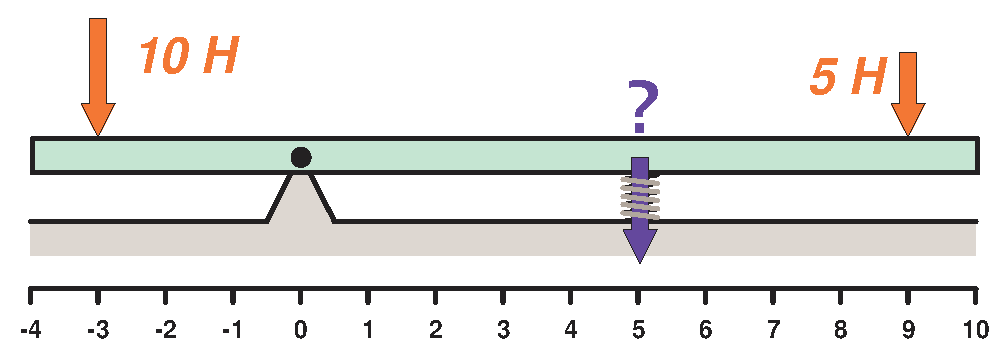
\includegraphics{GP005F03.eps}}
  \end{picture}\\
Задачка: какое усилие испытывают динамометр и ось рычага?\\
Решение: \begin{itemize}
\item момент правой силы $=\mathcal{M}_1=9\cdot5=+45$
\item момент левой силы $=\mathcal{M}_2=(-3)\cdot10=-30$
\item суммарный момент $=\mathcal{M}_\Sigma=\mathcal{M}_1+\mathcal{M}_2=+15$
\item сила на динамометре $F_\texttt{д}=\mathcal{M}_\Sigma/5=+3$ H
\item сила давления на ось $F_o=10+5-3=12$ H
\end{itemize}

Еще задачка: каков момент инерции различных простых тел?\\[2mm]
{\color{red} $\bullet$ Тонкий стержень} массой $m$ и длиной $2L$:\\
  \begin{picture}(190,20)(0,0)
   \linethickness{2mm}
   {\color{red}
   \put(30,10){\line(1,0){120}}
   }
   \put(120,10){\line(1,0){5}}
   \linethickness{0.01in}
   \put(90,10){\circle{5}}
   \put(90,10){\circle*{2}}
   \put(90,6){\vector(1,0){30}}
   \put(30,8){\makebox(0,0)[t]{\color{red}\bf -L}}
   \put(150,8){\makebox(0,0)[t]{\color{red}\bf +L}}
   \put(122,6){\makebox(0,0)[l]{$r$}}
   \put(123,12){\makebox(0,0)[b]{$dr$}}
  \end{picture}\\
Разделим стержень на кусочки. Пусть один такой кусочек длиной $dr$ находится от оси вращения на расстоянии $r$. Его масса $dm=m\cdot dr/2L$, а момент инерции $d\mathcal{I}=r^2\,dm=
mr^2dr/2L$. Момент инерции всего стержня равен
\begin{displaymath}
\mathcal{I}=2\int_0^Lm\frac{r^2dr}{2L}={\color{red}\frac{1}3mL^2}.
\end{displaymath}
{\color{red} $\bullet$  Тонкостенный цилиндр} массой $m$ и радиусом $R$:\\
  \begin{picture}(190,35)(0,0)
   %\put(0,0){\framebox(190,40)[b]{}}
   \put(0,0){\includegraphics{GP005F04.eps}}
   \put(190,5){\makebox(0,0)[br]{\parbox{135mm}{Разобьем цилиндр на полоски с массой по $\Delta m_i$. \\
Момент инерции полоски $\Delta\mathcal{I}_i=\Delta m_iR^2$. \\
Момент инерции всего цилиндра $\mathcal{I}=\sum\Delta\mathcal{I}_i=\\ \sum\Delta m_iR^2=R^2\sum\Delta m_i=\color{red}mR^2$.
   }}}
  \end{picture}\\
{\color{red} $\bullet$  Cплошной цилиндр} представим как набор полых цилиндриков с радиусами r от 0 до R и толщинами dr. Тогда масса каждого цилиндрика будет $dm_i=m\cdot\frac{2\pi r\cdot dr}{\pi R^2}$, а суммарный момент инерции, соответственно --\vspace{-2mm}
\begin{displaymath}
\int_0^m r^2 dm = \int_0^R r^2m\frac{2 r\cdot dr}{R^2}=\frac{2m}{R^2}\int_0^Rr^3dr=\frac{2m}{R^2}\frac{R^4}4=\color{red}\frac12mR^2
\end{displaymath}
{\color{red} $\bullet$ Сфера}: разобьем ее на кольца сечением $R\,d\theta$ и длиной $2\pi h=2\pi\,R\,\sin\theta$.\\
  \begin{picture}(190,40)(0,0)
   %\put(0,0){\framebox(190,38)[b]{}}
   \put(0,0){\includegraphics{GP005F05.eps}}
   \put(190,-5){\makebox(0,0)[br]{\parbox{150mm}{Площадь одного кольца $dS=2\pi R^2\sin\theta\,d\theta$, его масса $dm=m\frac{dS}S=m\,(2\pi R^2\sin\theta\,d\theta)/(4\pi R^2)=m\,\sin\theta\,d\theta/2$, а момент инерции
$d\mathcal{I}=h^2\,dm=\frac{mR^2}2\sin^3\theta\,d\theta$. Для всей сферы:\vspace{-3mm}
\begin{displaymath}
\mathcal{I}=\int_0^\pi\frac{mR^2}2\sin^3\theta\,d\theta=
\frac{mR^2}2\frac{4}3={\color{red}\frac{2}3mR^2}
\end{displaymath}
   }}}
  \end{picture}
{\color{red} $\bullet$ Однородный шар}: выделим кольцо сечением $rd\theta\times dr$ и длиной $2\pi h$=\\
\begin{picture}(190,70)(0,0)
   %\put(0,0){\framebox(190,70)[b]{}}
   \put(0,0){\includegraphics{GP005F06.eps}}
   \put(190,68){\makebox(0,0)[tr]{\parbox{120mm}{$=2\pi\,r\,\sin\theta$.
Объем одного такого кольца $dV=2\pi r^2\sin\theta\,d\theta\,dr$. Поскольку шар однороден, то масса кольца $dm$ пропорциональна $dV$ и равна
\begin{displaymath}
 dm=m\frac{dV}V=m\,\frac{2\pi r^2\sin\theta\,d\theta\,dr}{4\pi R^3/3},
\end{displaymath}
а момент инерции кольца $d\mathcal{I}$ составляет
\begin{displaymath}
d\mathcal{I}=h^2\,dm=m\,\frac{3 r^4\sin^3\theta\,d\theta\,dr}{2 R^3}
\end{displaymath}
   }}}
  \end{picture}\\
Чтобы получить суммарный момент инерции всего шара, надо проинтегри\-ровать $d\mathcal{I}$ по $\theta$ от 0 до $\pi$ и по $r$ от 0 до $R$:
\begin{displaymath}
\mathcal{I}=\int_0^\pi \int_0^R d\mathcal{I}=\frac{3m}{2 R^3}\int_0^\pi\sin^3\theta\,d\theta \int_0^Rr^4\,dr
\end{displaymath}
Второй из нтегралов равен $R^5/5$, а для вычисления первого сделаем замену: $x\equiv-\cos\theta$. Тогда $dx=\sin\theta$, а $\sin^2\theta=(1-x^2)$, и, как и для сферы,
\begin{displaymath}
\int_0^\pi\sin^3\theta\,d\theta = \int_{-1}^1(1-x^2)dx = \left.\left(x-\frac{x^3}3\right)\right|_{-1}^1=\frac 43
\end{displaymath}
Подставив значения обоих интегралов, получим:
\begin{displaymath}
\mathcal{I}=\frac{3mR^5\cdot4}{2 R^3\cdot5\cdot3}={\color{red}\frac 25mR^2}
\end{displaymath}
\begin{picture}(190,50)(0,0)
   %\put(0,0){\framebox(190,50)[b]{}}
   \put(0,0){\includegraphics{GP005F07.eps}}
   \put(190,50){\makebox(0,0)[tr]{\parbox{130mm}{
   Поворот тела на угол $\varphi$ вокруг внешней оси эквивалентен поступательному движению по дуге и повороту относительно собственной оси на тот же угол $\varphi$. При этом, для поступательного движения важен только центр масс тела, а для вращения -- его собственный момент инерции $\mathcal{I}_0$.
   }}}
\end{picture}\\
\underline{Теорема Штейнера:} Момент инерции тела $\mathcal{I}$ относительно какой-либо оси равен сумме собственного момента инерции $\mathcal{I}_0$ (относительно параллельной оси, но проходящей через его центр масс) и момента инерции центра масс:
\begin{displaymath}
\mathcal{I}=\mathcal{I}_0+MR_C^2
\end{displaymath}
\begin{picture}(190,50)(0,0)
   %\put(0,0){\framebox(190,50)[b]{}}
   \put(70,0){\includegraphics{GP005F08.eps}}
   \put(0,50){\makebox(0,0)[tl]{\parbox{65mm}{
   Задача: найти момент инерции гантели (2 шара радиусами $R$ и массами $M$ на расстоянии $4R$ друг от друга)
   }}}
\end{picture}\\
Решение: собственный момент инерции каждого из двух шаров $\mathcal{I}_0=MR^2\cdot2/5$, а момент инерции центра масс каждого шара относительно оси $\mathcal{I}_C=M(2R)^2=4MR^2$. Итого, в сумме получается:
\begin{displaymath}
\mathcal{I}=2\mathcal{I}_0+2\mathcal{I}_C=8.8\,MR^2
\end{displaymath}
Если гантель вращается с угловой скоростью $\omega$, то какова энергия вращения? Каждый элемент с массой $\Delta m_i$ имеет одну и ту же угловую скорость $\omega$, но линейные скорости $v_i$ будут различны: $v_i=r_i\omega$. Кинетическая энергия каждого кусочка будет $\Delta E_i=\Delta m_iv_i^2/2=\omega^2/2\cdot\Delta m_ir_i^2$, а энергия всего тела --
\begin{displaymath}
E_\texttt{rot}=\sum_i\Delta E_i=\omega^2/2\cdot\sum_i\Delta m_ir_i^2
\end{displaymath}
Но последняя сумма -- это же момент инерции! Таким образом, действительно
\begin{displaymath}
E_\texttt{rot}=\frac{\mathcal{I}\omega^2}2
\end{displaymath}

Пусть по наклонной плоскости без трения скатываются: 1) пустая бочка, 2) бочка со смолой и 3) бочка с водой. Которая скатится быстрее?

У всех потенциальная энергия $mgh$ переходит в кинетическую, состоя\-щую из энергии поступательного движения $mv^2/2$ и энергии вращения $\mathcal{I}\omega^2/2$. Для катящейся бочки ее линейная и угловая скорости связаны как $v=R\omega$, поэтому для каждой из них справедливо уравнение\vspace{-2mm}
\begin{displaymath}
mgh=\frac{mv^2}2+\frac{\mathcal{I}v^2}{2R^2}
\end{displaymath}\vspace{-2mm}
Полагая пустую бочку тонкостенным цилиндром, вспоминаем, что в этом случае $\mathcal{I}=mR^2$. Для бочки со смолой, эквиваленитной сплошному цилин\-дру, $\mathcal{I}=\frac 12mR^2$. Бочка же с водой -- это особый случай. Считая вязкость воды бесконечно малой, а массу намного большей, чем масса самой бочки, можно заявить, что вода внутри вообще не крутится, и что энергией вращения можно пренебречь.

Тогда для трех бочек получаем три разные уравнения:
\begin{displaymath}
\begin{array}{ll}
1)\rule{10mm}{0mm} mgh=\frac{mv^2}2+\frac{mv^2}2&
  \hspace{10mm}\Rightarrow\hspace{10mm}v^2=gh\\
2)\rule{10mm}{0mm} mgh=\frac{mv^2}2+\frac{mv^2}4&
  \hspace{10mm}\Rightarrow\hspace{10mm}v^2=1.5gh\\
3)\rule{10mm}{0mm} mgh=\frac{mv^2}2+0&
  \hspace{10mm}\Rightarrow\hspace{10mm}v^2=2gh
\end{array}
\end{displaymath}

\underline{\bf Гироскоп}\\
\begin{picture}(190,35)(0,0)
   %\put(0,0){\framebox(190,35)[b]{}}
   \put(0,0){\includegraphics{GP005F9a.eps}}
   \put(135,0){\includegraphics{GP005F9b.eps}}
   \put(95,35){\makebox(0,0)[t]{\parbox{65mm}{
   Приложим к гироскопу пару сил {\color{red}$\vec{F}\vec{F'}$}, создающих момент {\color{red}$\vec{M}$}. Он создаст угловое ускорение {\color{blue}$\vec{\beta}=\dot{\vec{\omega}}$},
   }}}
   \put(95,0){\makebox(0,0)[b]{которое за малый отрезок времени $\Delta t$}}
\end{picture}\\
изменит угловую скорость {\color{blue}$\vec{\omega}$} на приращение {\color{blue}$\vec{\Delta\omega}$} и тем самым повернет ось вращения вовсе не туда, куда тянули ее силы {\color{red}$\vec{F}\vec{F'}$}! Это и есть {\bf гиро\-ско\-пи\-че\-ский эффект}.

Использование: стабилизация и/или ориентация в пространстве (ги\-ро\-компасы, нарезное огнестрельное оружие, орудия в танках и на флоте, ста\-би\-ли\-зация аэрокосмических аппаратов).

{\bf Прецессия} -- круговое смещение оси вращения под действием посто\-ян\-ного опрокидывающего момента. Ядерный магнитный резонанс (ЯМР).
\end{document} 